\section{Data}
\label{sec:data}

For this work we utilise a sample of 68 PSBs drawn from the SDSS-IV MaNGA (Mapping Nearby Galaxies at Apache Point Observatory) integral field spectroscopic survey. The PSB sample comprises 31 CPSBs and 37 RPSBs. This sample, and a control sample of approximately 480 normal galaxies (that is not exhibiting PSB regions),  were kindly provided by Chen et al. (2019, submitted).

\subsection{The SDSS-IV MaNGA survey}
\label{sec:MaNGA}
The data used in this work includes galaxy stellar velocity and gas velocity kinematic maps, spectral index maps and individual spectra drawn from the Sloan Digital Sky Survey (SDSS) phase IV project MaNGA (Mapping Nearby Galaxies at Apache Point Observatory). An overview of the SDSS-IV MaNGA project is provided by \citet{2015ApJ...798....7B}, where key instrumentation features and observational strategy are described. MaNGA captures dithered observations with 17 fibre-bundle integral
field units (IFUs) that vary in size from 19 fibres to 127 fibres (3-7 hexagonal layers). Two dual-channel spectrographs provide
simultaneous wavelength coverage over the range 3600 to 10300 \AA\ at a spectral resolution of R$\sim$2000. MaNGA is an integral field spectroscopic survey (IFS) which provides spatially resolved properties of galaxies and can provide evidence of external influences such as close neighbour interaction, present merger activity and the signatures of past merger history.

IFU dithered data are processed in the MaNGA Data Reduction Pipeline (DRP) to produce calibrated spectra and rectified three-dimensional data cubes. The final data products of the DRP feed into the MaNGA data analysis pipeline (DAP) \citep{2016AJ....152...83L,2019arXiv190100856W} which, the purposes of this paper, provides:
\begin{itemize}
    \item Spatially stacked spectra
    \item Stellar kinematics (velocity, V, and velocity dispersion, $\sigma$)
    \item Nebular emission-line properties: fluxes, equivalent widths, and kinematics (V and $\sigma$)
    \item Spectral Indices: absorption-line (e.g.  H$\delta_A)$ and bandhead (e.g., D$_n$4000) measurements
\end{itemize}

Kinematic data is extracted from the MaNGA DAP output DAPTYPE MAPS-SPX-GAU-MILESHC: where SPX denotes individual spaxel binning; GAU a Gaussian fit algorithm to stellar spectra; and MILESHC is a reference to the MILES library \citep{2011A&A...532A..95F} of stellar spectrum templates, all as described in the MaNGA DR15 DAP documentation \citet{2019arXiv190100856W}. The 2-D maps provide the following data: 

\begin{itemize}
    \item Projected stellar rotation velocity
    \item Stellar velocity dispersion
    \item Ionised gas rotational velocity
    \item Ionised gas velocity dispersion
\end{itemize}

The associated 3-D datacubes MAPS-VOR10-GAU-
MILESHC provide spatial spectral series yielding the following spectral properties across the galaxy field-of-view:

\begin{itemize}
    \item D$_n$4000 spectral index as a measure of the strength of the 4000 \AA\ break
    \item H$\delta_A$ absorption spectral index
    \item Nebular emission line equivalent widths
\end{itemize}

The above datasets in the form of 3-D (2 spatial dimensions and 1 spectral wavelength dimension) datacubes can be downloaded from the SDSS science archive server (SAS) or by using the Marvin web interface tool\footnote{https://dr15.sdss.org/marvin/} as described in \cite{2018arXiv181203833C}. SDSS and MaNGA data is released periodically in MaNGA Product Launches (MPL) each with an accompanying data release (DR) number. DR15 is the third data release of the the fourth phase of the SDSS observational programme and includes all data from prior releases. In this project we use MaNGA MPL-7, DR15 datacubes \citep{2019ApJS..240...23A}. The associated FITS-format galaxy data summary table output from DRP \texttt{drpall} file is version 2.4.3 \citep{2016AJ....152...83L}. The important \texttt{drpall} data fields for this project are listed in Table \ref{tab:DRPall-table}.

\begin{table*}
\caption[MaNGA DRPALL fields used in the project]{SDSS-IV MaNGA DRPALL v2.4.3 data fields used in the project}
\label{tab:DRPall-table}
\begin{tabular}{|p{3.2cm}|p{1.2cm}||p{1cm}|p{10cm}|}
\hline
Name & Type & Unit & Description \\
\hline
PLATEIFU & char{[}100{]} &  & Plate+ifudesign name for this object (e.g. 7443-12701)\\
MANGAID & char{[}100{]} & & MaNGA ID for this object (e.g. 1-114145)\\
OBJRA & float64 & degrees & Right ascension of the science object in J2000\\
OBJDEC & float64 & degrees & Declination of the science object in J2000\\
NSA\_Z & float64 &  & Heliocentric redshift\\
NSA\_ZDIST & float64 &  & Distance estimate using peculiar velocity model of Willick et al. (1997); mulitply by c/Ho for Mpc\\
NSA\_ELPETRO\_MASS & float64 &  & Stellar mass from K-correction fit (use with caution) for elliptical Petrosian fluxes ($\Omega_m=0.3$, $\Omega_\Lambda=0.7$, $h=1$)\\
NSA\_ELPETRO\_BA & float64 &  & Axis ratio used for elliptical apertures (for this version, same as ba90)\\
NSA\_ELPETRO\_TH50\_R & float64 & arcsec & Elliptical Petrosian 50\% light radius in SDSS r-band\\
NSA\_SERSIC\_N & float64 &  & Se
rsic index from two-dimensional, single-component Sersic fit in r-band\\
\hline
\end{tabular}
\end{table*}

\subsection{Sample selection}
As noted in the introduction post-starburst galaxies or PSB regions of galaxies can be identified from their spectra which typically exhibit the strong Balmer absorption lines of A-type stars, and in addition, weak H$\alpha$ and/or [OII] emission lines which indicate a quiescent state with little or no present star formation. 

The PSB and control samples provided by Chen et al. (2019, submitted, personal communication) was drawn from an analysis of 4633 galaxies made available as MPL-6 (SDSS-IV MaNGA Product Launch 6) The objective was to select PSB regions that have recently and rapidly quenched their star formation.  To achieve this goal Chen et al. (2019, submitted) adopted the following sample selection criteria:
\begin{itemize}
    \item Spaxels with signal-to-noise S/N > 10 per pixel
    \item Strong H$\delta_A$ absorption line > 3\AA 
    \item A strong 4000 \AA\ break 
    \item Weak H$\alpha$ equivalent width W(H$\alpha$) < 10\AA
    \item and $\log{W(H\alpha)} < 0.23\times{H\delta_A}-0.46$
\end{itemize}
The H$\delta_A$ absorption spectral index is the equivalent width of H$\delta$ 4102\AA\ line as described by \citet{1994ApJS...94..687W}. In addition to the above criteria, for a region to be classed as PSB at least 6 contiguous spaxels from the DAP analysis are required. To put the above selection criteria in context with the SDSS-IV MaNGA datacube output, example maps of D$_n$4000 spectral index, H$\delta_A$, and H$\alpha$ equivalent width W(H$\alpha$) are shown in Figure [TODO]. 

Using an earlier data release, MaNGA major product launch  MPL-6\footnote{https://sdss-marvin.readthedocs.io/en/stable/datamodel/mpl6.html}, Chen et al. (2019, submitted) identified 360 galaxies possessing PSB spaxel regions meeting the above selection criteria. They then categorised the galaxies into 3 PSB types: those with central PSB regions (CPSBs); those with off-centre ring-like, or partial ring-like PSB features (RPSBs) and those with irregular regions of PSB spaxels in the outskirts (irregular PSBs or IPSBs). The PSB selection from Chen et al. (2019) yielded a total of 31 CPSBs and 37 RPSBs. Useful data from the MaNGA \texttt{drpall} file for these selected PSBs are listed in appendix \ref{sec:lists-of-psbs}, Tables \ref{tab:my-CPSBs} and \ref{tab:my-RPSBs} respectively. We will use the data in these tables frequently throughout this report to investigate the distribution of various parameters between the PSB groups and their control samples.

The distribution of the CPSB and RPSB samples is shown in a colour-mass plot in Figure \ref{fig:Colour-Mass-PSBs}. The contour plot represents the complete MaNGA DR15 population plotted as the NSA (NASA Sloan atlas) colour index NUV-i values versus galaxy stellar mass obtained from the NSA data field  NSA\_ELPETRO\_LOGMASS. Our PSB samples are superimposed on the DR15 density contour plot. We note that the population of CPSBs generally lie redward of the RPSBs in the colour-mass diagrams of Figures \ref{fig:Colour-Mass-PSBs}. The mass distributions of the two PSB populations are similar, however.

\begin{figure}
    \centering
    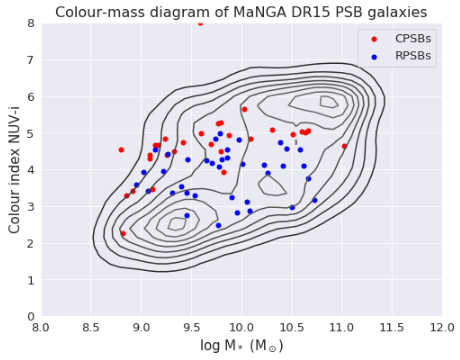
\includegraphics[width=\columnwidth]{images/CMDs/CMD-PSBs-CONTOUR-TIX.png}
    \caption[Colour-mass distribution of PSBs]{The sample of PSB galaxies is shown distributed over the complete DR15 population density contour plot as shown in Figure \ref{fig:CMD-mass-1}. CPSBs are represented by red dots and RPSBs as blue dots.}
    \label{fig:Colour-Mass-PSBs}
\end{figure}

\subsection{Control galaxies}
\label{sec:controls}
A control sample set of regular galaxies not exhibiting PSB features was selected by Chen et al. (2019) sample. The purpose of the control sample is to provide a reference set of properties for comparison with the PSB data with a view to identifying typical progenitors which have not (yet) experienced a major merger. For each PSB, (CPSBs and RPSBs), a set of 10 non-PSB galaxies were selected but having similar stellar mass and global D$_n$4000 spectral indices. We used this control galaxy sample in this work.

Colour-mass diagrams of the two PSB groups with subsets of their control group samples are presented in Figure \ref{fig:Colour-Mass-PSBs-controls}. The colour-mass distribution of each of the PSB groups, CPSBs and RPSBs, is generally similar to that of their respective control groups. This confirms that the general objectives of control selection was achieved.

\begin{figure*}
    \centering
    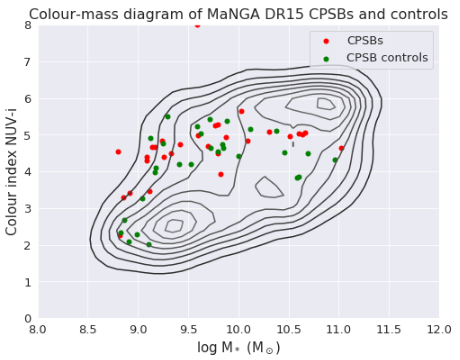
\includegraphics[width=\columnwidth]{images/CMDs/CMD-CPSBs+CONTROLS-TIX.png}
    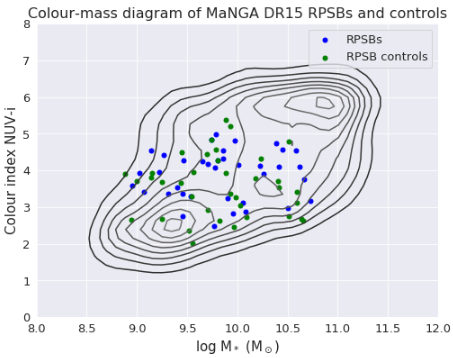
\includegraphics[width=\columnwidth]{images/CMDs/CMD-RPSBs+CONTROLS-TIX.png}
    \caption[Colour-mass distribution of PSBs and controls]{The contents are similar to Figure \ref{fig:Colour-Mass-PSBs}. The colour-mass distribution of PSBs and their control galaxies has been superimposed on the contour plot of the complete DR15 population. The left panel shows the distribution of the CPSB sample (red dots) with their control galaxies (green dots), in the right panel the RPSB sample (blue dots) with their corresponding controls (again with green dots).}
    \label{fig:Colour-Mass-PSBs-controls}
\end{figure*}

\subsection{PSB spectra}
The spectrum of a PSB galaxy exhibiting central PSB features is shown in Figure \ref{fig:CPSB-8623-9102-spec}.
\begin{figure*}
    \centering
    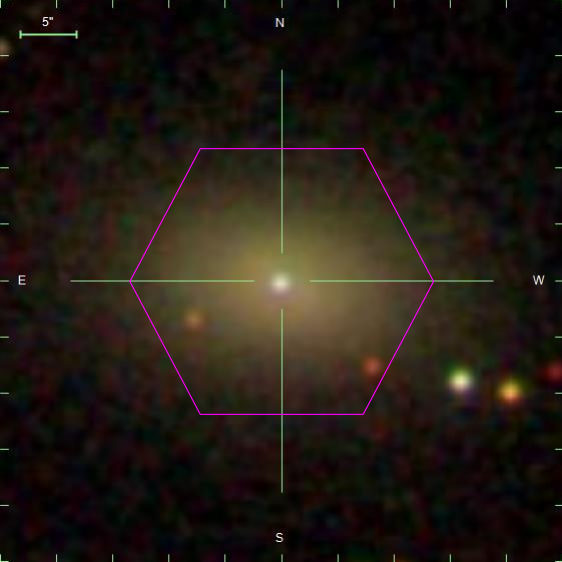
\includegraphics[width=0.22\textwidth]{images/Cutouts/CPSB-8623-9102-IM.png}
    \hfill
    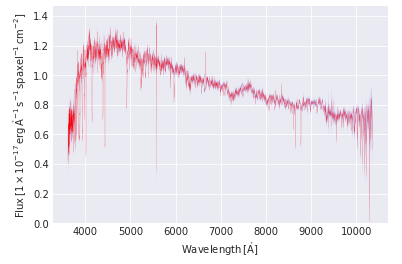
\includegraphics[width=0.38\textwidth]{images/Spectra/CPSB-8623-9102.png}
    \hfill
    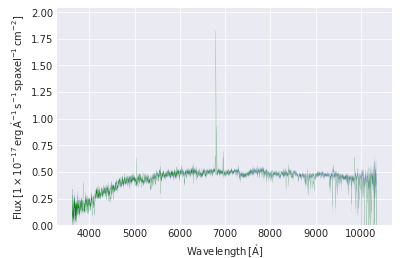
\includegraphics[width=0.38\textwidth]{images/Spectra/CPSB-CTRL-8990-3703-spec.png}
    \caption[Central spaxel spectrum of CPSB 8623-9102]{Left: SDSS 3-colour image of central-type PSB 8623-9102. 
    Centre: The spectrum of the central spaxel of CPSB  8623-9102. Note the Balmer break feature and strong hydrogen absorption lines in the wavelength region 3500 to 4500 \AA.
    Right: For comparison with the centre panel, the centre spaxel spectrum of control galaxy 8990-3703 (having similar stellar mass to 8623-9102). The central spaxel spectrum of this is control galaxy shows relatively weak absorption lines and exhibits a strong H$\alpha$ emission line indicating the presence of ongoing star formation.}
    \label{fig:CPSB-8623-9102-spec}
\end{figure*}


The spectrum obtained from the central spaxel of a ring-type RPSB galaxy is shown in Figure \ref{fig:RPSB-8323-6103-spec}. The central spectrum obtained at spaxel coordinates [27,27] shows strong H$\alpha$ emission consistent with the presence of an ample gas supply for continuing star formation. Moving away from the central spaxel, in the direction towards the upper right of the IFU frame, the spectrum at spaxel coordinates [34,32] exhibits the characteristics of a post-starburst region. The spectrum reveals weak emission lines and strong Balmer absorption lines typical of the stellar atmospheres of A-type stars. This indicates the presence of a ring-type PSB feature at this location.

\begin{figure*}
    \centering
    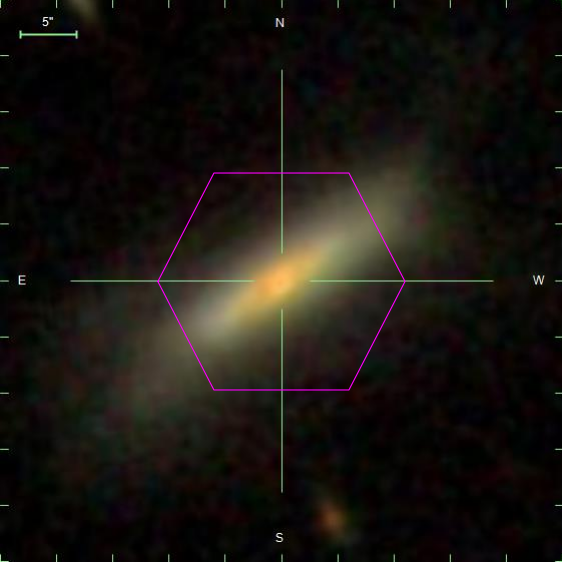
\includegraphics[width=0.24\textwidth]{images/Cutouts/RPSB-8323-6103-IM.png}
    \hfill
    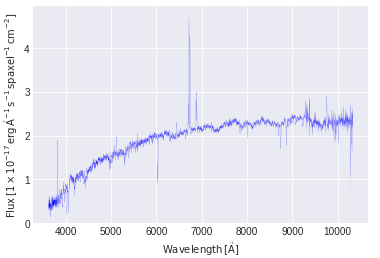
\includegraphics[width=0.35\textwidth]{images/Spectra/RPSB-8323-6103-27-27.png}
    \hfill
    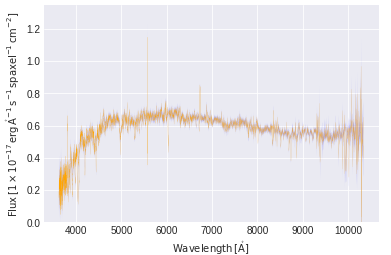
\includegraphics[width=0.35\textwidth]{images/Spectra/RPSB-8323-6103-34-32.png}
    \caption[Image and central and offset spectra of the RPSB 8323-6103]{The gri image, central and offset spectra of the RPSB 8323-6103. Left: SDSS 3-colour image of the ring-type PSB 8323-6103. 
    Centre: spectrum of the central region of ring-type PSB 8323-6103 at spaxel coordinates [27, 27] reveals strong H$\alpha$ emission. 
    Right: spectrum of ring-type PSB 8323-6103 at spaxel coordinates [34, 32], this location is above and to the right of centre. The spectra in spaxels nearby this location exhibit post-starburst features of weak emission lines and strong Balmer absorption lines.}
    \label{fig:RPSB-8323-6103-spec}
\end{figure*}

\subsection{Velocity maps}
Our kinematic studies employ stellar and gas velocity maps obtained from SDSS MaNGA datacubes. Examples of MaNGA stellar velocity and gas velocity maps for the CPSB 8313-6101 is illustrated in Figure \ref{fig:CPSB-8313-6101-VMAPS}. In our kinematic analysis we are looking for anomalies in the velocity fields, such as non-linear radial variation, which may provide evidence of past merger activity.

\begin{figure*}
    \centering
    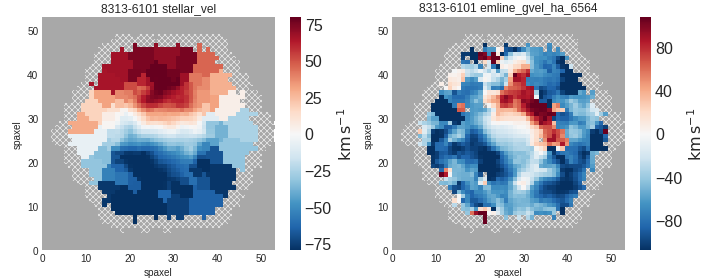
\includegraphics[width=0.9\textwidth]{images/VelocityMaps/CPSB-8313-6101-VMAPS.png}
    \caption[MaNGA velocity maps for CPSB 8313-6101]{MaNGA velocity maps for CPSB 8313-6101: stellar velocity (left) and H$\alpha$ gas velocity (right).}
    \label{fig:CPSB-8313-6101-VMAPS}
\end{figure*}



